\chapter{2026年云南}
\begin{enumerate}
\item
%% number: 1
%% paperName: 2026年云南高考第 1 题 4 分
%% typeId: 1
%% type: 单选题
%% chapter: 光学
%% point: 光电效应
%% method: 无
%% score: 4
%% degree: 950
%% duplicateId: 0
%% body:
云南省锡、铟等有色金属储量丰富。已知锡和铟的逸出功分别为 $ 4.42 \UeV $ 和 $ 4.09 \UeV $，若用光子能量为 $ 4.30 \UeV $ 的紫外线分别照射这两种金属，则 \xzanswer{B}


\fourchoices[answer=B]
{只有锡能发生光电效应}
{只有铟能发生光电效应}
{锡和铟都能发生光电效应}
{锡和铟都不能发生光电效应}

%% answer: B

\item
%% number: 2
%% paperName: 2026年云南高考第 2 题 4 分
%% typeId: 1
%% type: 单选题
%% chapter: 运动和力
%% point: 超重失重
%% method: 无
%% score: 4
%% degree: 850
%% duplicateId: 0
%% body:
云南宣威尼珠河大峡谷的“青云电梯”为谷底孩子们上学提供了交通便利。若电梯由静止开始上升 $ 260 \Um $，用时 $ 100 \Us $，则此过程电梯的平均速度大小及电梯向上加速时乘客所处的状态分别为 \xzanswer{A}


\fourchoices[answer=A]
{$ 2.6 \Ums $，超重}
{$ 0.38 \Ums $，超重}
{$ 2.6 \Ums $，失重}
{$ 0.38 \Ums $，失重}

%% answer: A

\item
%% number: 3
%% paperName: 2026年云南高考第 3 题 4 分
%% typeId: 1
%% type: 单选题
%% chapter: 光学
%% point: 光的折射
%% method: 无
%% score: 4
%% degree: 850
%% duplicateId: 0
%% body:
在测量某种透明树脂折射率的实验中，让激光束射入一块两面平行的树脂砖，改变入射点和入射角，得到①、②、③、④四条出射光线，如图所示。不考虑反射，图中经 $ P $ 点射入树脂砖的光，出射后的光线可能是 \xzanswer{B}
\begin{figure}[htbp]
	\centering
	\includesvg[width=202.5pt,height=154.5pt]{pic/2026/云南/01}
\end{figure}

\fourchoices[answer=B]
{①}
{②}
{③}
{④}

%% answer: B

\item
%% number: 4
%% paperName: 2026年云南高考第 4 题 4 分
%% typeId: 1
%% type: 单选题
%% chapter: 曲线运动
%% point: 开普勒定律
%% method: 无
%% score: 4
%% degree: 650
%% duplicateId: 0
%% body:
我国“天宫”空间站的轨道离地高度约为 $ 400 \Ukm $，空间站内的宇航员每 $ 24 \Uh $ 能看到 $ 16 $ 次日出。“吉林一号”遥感卫星组网中的某颗卫星轨道离地高度约为 $ 535 \Ukm $。已知地球半径约为 $ 6400 \Ukm $，空间站与该卫星绕地球的运动均视为匀速圆周运动，则该卫星的周期约为 \xzanswer{B}


\fourchoices[answer=B]
{$ 1.0\Uh $}
{$ 1.5\Uh $}
{$ 2.0\Uh $}
{$ 2.4\Uh $}

%% answer: B

\item
%% number: 5
%% paperName: 2026年云南高考第 5 题 4 分
%% typeId: 1
%% type: 单选题
%% chapter: 机械波
%% point: 波长频率波速
%% method: 无
%% score: 4
%% degree: 550
%% duplicateId: 0
%% body:
如图所示，均匀介质中的三个质点 $ S $、$ P $、$ Q $，它们分别静止于直角坐标系 $ Oxy $ 平面内的（$ 0 $，$ 0 $）、（$ - 2 $，$ 0 $）和（$ 4 $，$ 3 $）处。$ t =0 $ 时刻，$ S $ 从平衡位置开始垂直 $ Oxy $ 平面向上振动，振动频率为 $ 2 \UHz $，形成向外传播的简谐横波，图中实线圆表示某时刻相邻的两个波峰，则 \xzanswer{C}
\begin{figure}[htbp]
	\centering
	\includesvg[width=165.0pt,height=126.8pt]{pic/2026/云南/02}
\end{figure}

\fourchoices[answer=C]
{该波的波速大小为 $ 8 \Ums $}
{$ t =0.125 \Us $ 时，$ P $ 位于波峰}
{该波传播到 $ P $、$ Q $ 的时间差为 $ 0.75 \Us $}
{$ t =1.25 \Us $ 以后，$ P $、$ Q $ 的位移始终相同}

%% answer: C

\item
%% number: 6
%% paperName: 2026年云南高考第 6 题 4 分
%% typeId: 1
%% type: 单选题
%% chapter: 力物体的平衡
%% point: 动态平衡
%% method: 无
%% score: 4
%% degree: 450
%% duplicateId: 0
%% body:
如图所示，两挂钩可沿固定水平横梁滑动到任意位置后锁定。一挎包质量为 $ m $，其轻质包带长度约为 $ 4 d $，$ a $、$ b $ 为包与包带的连接点，相距为 $ d $。将挎包悬挂在两挂钩上，两挂钩相距为 $ x $ 时，锁定挂钩。挎包静止时，$ a $、$ b $ 在同一水平直线上，包带的张力大小为 $ F_{T} $，重力加速度为 $ g $，不计包带与挂钩之间的摩擦及两挂钩尺寸。能正确反映$ \frac{{{F_{T}}}}{{mg}} $随 $ x $ 变化的图像是 \xzanswer{D}

\begin{figure}[htbp]
\centering
\includesvg[width=262.5pt,height=139.5pt]{pic/2026/云南/03}
\end{figure}
\fourchoices[answer=D,ispicture=true]
{\includesvg[height=78.1pt]{pic/2026/云南/04a}}
{\includesvg[height=78.1pt]{pic/2026/云南/04b}}
{\includesvg[height=78.1pt]{pic/2026/云南/04c}}
{\includesvg[height=78.1pt]{pic/2026/云南/04d}}



%% answer: D

\item
%% number: 7
%% paperName: 2026年云南高考第 7 题 4 分
%% typeId: 1
%% type: 单选题
%% chapter: 电场
%% point: 带电粒子的偏转
%% method: 无
%% score: 4
%% degree: 450
%% duplicateId: 0
%% body:
如图所示，在大小、方向均未知的匀强电场中，$ O $、$ M $、$ N $ 三点处于同一竖直面内，将一质量为 $ 0.1 \Ukg $、电荷量为 $ 1.0 \times 10 ^{-6} \UC $ 的带正电的小球（视为质点）从 $ O $ 点抛出，小球 $ 1 \Us $ 后到达 $ O $ 点正上方 $ 3m $ 处的 $ M $ 点，再经 $ 1 \Us $ 到达 $ N $ 点，$ O $、$ N $ 两点在同一水平线上且相距 $ 3m $。不计空气阻力，重力加速度 $ g $ 取 $ 10 \Ums ^{2} $，设电场强度大小为 $ E $，$ O $、$ N $ 两点的电势分别为 $ \varphi_{O} $ 和 $ \varphi_{N} $，则 \xzanswer{C}
\begin{figure}[htbp]
	\centering
	\includesvg[width=120.0pt,height=122.2pt]{pic/2026/云南/05}
\end{figure}

\fourchoices[answer=]
{$ E =6.7 \times 10 ^{5} \UVm $，$\varphi_{O} > \varphi_{N}$}
{$ E =6.7 \times 10 ^{5} \UVm $，$\varphi_{O} < \varphi_{N}$}
{$ E =5.0 \times 10 ^{5} \UVm $，$\varphi_{O} > \varphi_{N}$}
{$ E =5.0 \times 10 ^{5} \UVm $，$\varphi_{O} < \varphi_{N}$}

%% answer: C

\item
%% number: 8
%% paperName: 2026年云南高考第 8 题 6 分
%% typeId: 2
%% type: 多选题
%% chapter: 电磁感应
%% point: 远距离输电
%% method: 无
%% score: 6
%% degree: 750
%% duplicateId: 0
%% body:
云南至广东高压输电工程在调试阶段采用 $ 800 \UkV $ 高压输电，输送功率为 $ 2.6 \times 10 ^{9} W $，关于该输电线路，下列说法正确的是 \xzanswer{BD}


\fourchoices[answer=BD]
{输电电流为 $ 3.25 \times 10 ^{6} \UA $}
{输电电流为 $ 3.25 \times 10 ^{3} \UA $}
{若输送功率不变，提高输电电压，则输电损耗会增加}
{若输送功率不变，提高输电电压，则输电损耗会减小}

%% answer: BD

\item
%% number: 9
%% paperName: 2026年云南高考第 9 题 6 分
%% typeId: 2
%% type: 多选题
%% chapter: 曲线运动
%% point: 斜抛运动
%% method: 无
%% score: 6
%% degree: 450
%% duplicateId: 0
%% body:
如图所示，运动员在空场上将排球从 $ a $ 点击出，$ a $ 点与球网顶部 $ b $ 点的水平距离为 $ x $、竖直距离为 $ h $，排球被击出时速度大小为 $ v $、方向与重力方向之间的夹角为 $ \theta $（$ 0 {^\circ} < \theta <180 {^\circ} $）。将排球视为质点，其运动轨迹所在平面与球网平面垂直，不计空气阻力，不考虑擦网球。运动员某次以 $ \theta =90 {^\circ} $ 击球时，排球贴近$ b $点越过球网后正好落到对方场地的底线上，相对于此次击球，下列说法正确的是 \xzanswer{AC}

\begin{figure}[htbp]
\centering
\includesvg[width=337.5pt,height=126.0pt]{pic/2026/云南/06}
\end{figure}
\fourchoices[answer=AC]
{保持 $ v $、$ x $、$ h $ 不变，减小 $ \theta $，排球一定下网}
{保持 $ v $、$ x $、$ h $ 不变，增大 $ \theta $，排球一定不会出界}
{保持 $ \theta $ 不变，增大 $ x $ 同时减小 $ h $，排球不下网就一定出界}
{保持 $ x $、$ h $ 不变，同时增大 $ v $ 和 $ \theta $，排球从被击出到落地所需时间可能不变}

%% answer: AC

\item
%% number: 10
%% paperName: 2026年云南高考第 10 题 6 分
%% typeId: 2
%% type: 多选题
%% chapter: 电磁感应
%% point: 电磁感应能量分析
%% method: 无
%% score: 6
%% degree: 350
%% duplicateId: 0
%% body:
如图所示，光滑绝缘斜面固定在水平面上，与水平面交于 $ PQ $，倾角 $ \theta =30 \Udu $，斜面上矩形 $ MNPQ $ 区域存在垂直斜面向下、磁感应强度大小 $ B =0.5\UT $ 的匀强磁场（图中未画出）。单匝等腰梯形导线框 $ abcd $ 的下底 $ ab=1.2 \Um $，上底 $ cd=0.6 \Um $，$ \angle a=53 \Udu $，质量 $ m =0.5 \Ukg $，总电阻 $ R =0.12 \UO $。线框从斜面上高于 $ MN $ 的某处由静止释放，$ ab $ 边进入磁场时开始对线框施加外力 $ F $ 控制其运动，$ cd $ 边进入磁场时 $ ab $ 边未出磁场。线框始终沿斜面运动，$ ab $ 边始终与 $ MN $ 平行，速度方向始终与 $ ab $ 边垂直。取重力加速度大小 $ g =10 \Umsq $，$ \sin 53 \Udu =0.8 $，设 $ ab $ 边进入磁场时速度为 $ v_{0} $，在线框进入磁场的过程中 \xzanswer{}
\begin{figure}[htbp]
	\centering
	\includesvg[width=217.5pt,height=162.8pt]{pic/2026/云南/07}
\end{figure}

\fourchoices[answer=AD]
{若速度保持恒定，且 $ v_{0} =2.0 \Ums $，则线框中的感应电流方向为 $ abcda $}
{若速度保持恒定，且 $ v_{0} =2.0 \Ums $，则该过程中 $ F $ 对线框始终做正功}
{若感应电流恒定，且 $ F $ 对线框做的功 $ W = - 0.79 \UJ $，则 $ v_{0} =0.3 \Ums $}
{若感应电流恒定，且$ F $ 对线框做的功 $ W = - 0.79 \UJ $，则该过程的时间 $ t =1.5 \Us $}

%% answer: AD

\item
%% number: 11
%% paperName: 2026年云南高考第 11 题 6 分
%% typeId: 4
%% type: 实验题
%% chapter: 力物体的平衡
%% point: 验证平行四边形实验
%% method: 无
%% score: 6
%% degree: 650
%% duplicateId: 0
%% body:
某同学做力的合成实验，实验装置如图~\ref{2026云南08a} 所示，该装置中三根支撑脚 $ L $、$ M $、$ N $ 的高度可通过地脚螺钉调节。完成下列填空：
\begin{figure}[htbp]
\centering
\begin{subfigure}{0.35\linewidth}
	\centering
	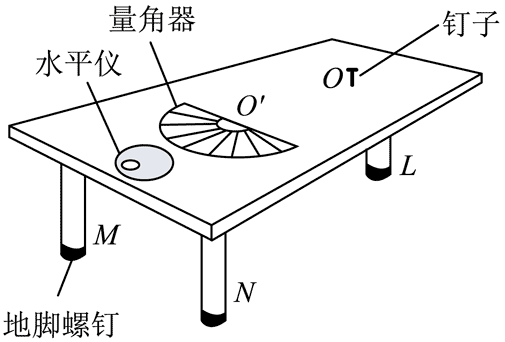
\includegraphics[height=3.3cm]{pic/2026/云南/08a.png}
	\caption{}\label{2026云南08a}
\end{subfigure}
\begin{subfigure}{0.2\linewidth}
	\centering
	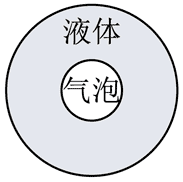
\includegraphics[height=1.8cm]{pic/2026/云南/08b.png}
	\caption{}\label{2026云南08b}
\end{subfigure}
\begin{subfigure}{0.35\linewidth}
	\centering
	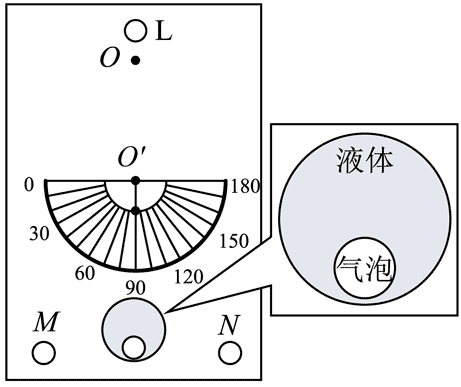
\includegraphics[height=3.3cm]{pic/2026/云南/08c.png}
	\caption{}\label{2026云南08c}
\end{subfigure}
\caption{}
\end{figure}
\begin{enumerate}
	\item 
该同学借助水平仪将实验装置台面调至水平。水平仪内封有液体和气泡，当水平仪底面水平时，气泡会静止在水平仪中心处，俯视图如图~\ref{2026云南08b} 所示。将水平仪放到台面上，气泡静止在水平仪中的位置俯视图如图~\ref{2026云南08c} 所示，下列操作能将台面调成水平的是 \tkanswer{A} 或 \tkanswer{D}（填正确答案标号）；

\fourchoices[answer=AD]
{保持 $ M $ 和 $ N $ 高度不变，调高 $ L $}
{保持 $ M $ 和 $ N $ 高度不变，调低 $ L $}
{保持 $ L $ 高度不变，同时调高 $ M $ 和 $ N $}
{保持 $ L $ 高度不变，同时调低 $ M $ 和 $ N $}


\item
如图~\ref{2026云南09a} 所示，将橡皮筋一端固定在 $ O $ 点，另一端通过圆环、细线与弹簧测力计相连。某次实验时，拉伸橡皮筋调整圆环圆心至 $ O '$ 点并保持静止，记录两细线的夹角，由弹簧测力计读出拉力 $ F_{1} $ 和 $ F_{2} $ 的大小，其中 $ F_{1} $ 的读数为 \tkanswer{$3.0$} $\UN[a]$；	


\begin{figure}[htbp]
	\centering
	\begin{subfigure}{0.35\linewidth}
		\centering
		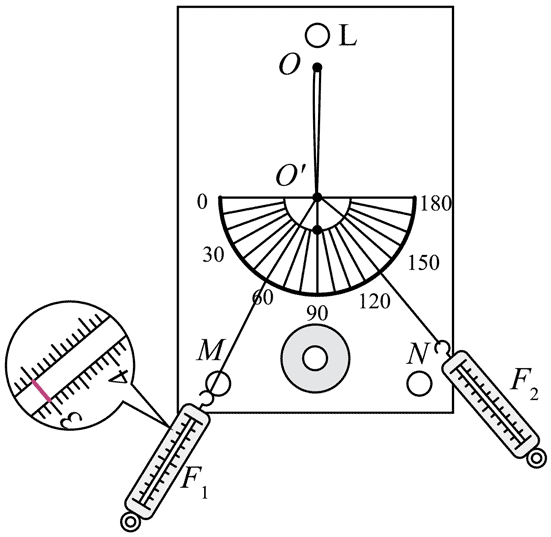
\includegraphics[height=3.9cm]{pic/2026/云南/09a.png}
		\caption{}\label{2026云南09a}
	\end{subfigure}
	\begin{subfigure}{0.25\linewidth}
		\centering
		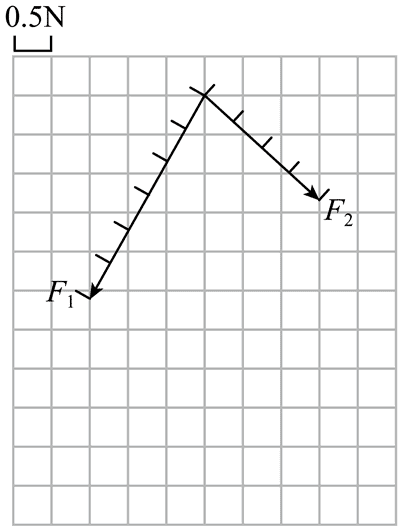
\includegraphics[height=3.9cm]{pic/2026/云南/09b.png}
		\caption{}\label{2026云南09b}
	\end{subfigure}
	\caption{}
\end{figure}

\item
根据测量结果在方格纸上画出 $ F_{1} $ 和 $ F_{2} $ 的图示，如图~\ref{2026云南09b} 所示。已知方格纸上每小格边长代表 $ 0.5 \UN $，用作图法可得 $ F_{1} $ 和 $ F_{2} $ 的合力大小为 \tkanswer{$4.0$} $\UN[a]$（结果保留 $ 2 $ 位有效数字）。

\end{enumerate}


%% answer:
\jdanswer{
\begin{enumerate}
	\item 
	A，D
	
	\item
	$3.0$
	
	\item
	$4.0$
\end{enumerate}
}
%% memo:
\memoanswer{
\begin{enumerate}
	\item 
水平仪气泡会向较高的一端移动，根据图丙可知是$ M $和$ N $端高了的原因，所以要将台面调成水平，需要保持 $ M $ 和 $ N $ 高度不变，调高 $ L $ 或者保持 $ L $ 高度不变，同时调低 $ M $ 和 $ N $，故选 $ A $ 或 $ D $。

\item
由图可知 $ F_{1} $ 的读数为 $ 6 \times 0.5 \UN=3.0 \UN $

\item
根据平行四边形法则做出合力图像如图所示
\begin{center}
	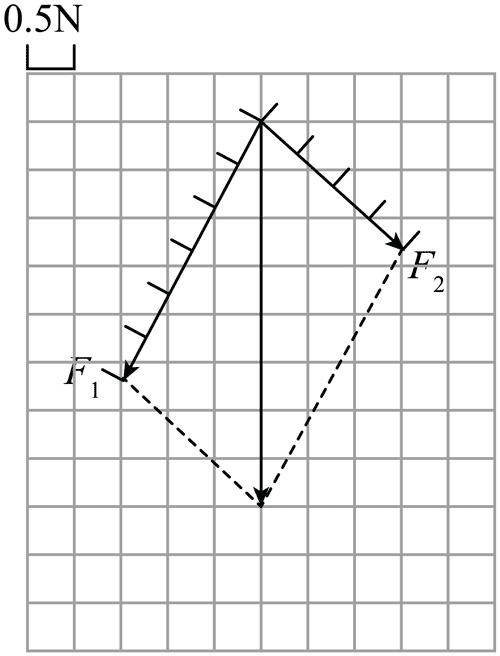
\includegraphics[width=135.0pt,height=177.0pt]{pic/2026/云南/10.png}
\end{center}
由于每小格边长代表 $ 0.5 \UN $，故可得 $ F_{1} $ 和 $ F_{2} $ 的合力大小为 $ F =8 \times 0.5N=4.0 \UN $
\end{enumerate}
}

\item
%% number: 12
%% paperName: 2026年云南高考第 12 题 10 分
%% typeId: 4
%% type: 实验题
%% chapter: 电路
%% point: 测电动势与内阻
%% method: 无
%% score: 10
%% degree: 450
%% duplicateId: 0
%% body:
某同学购买的蓝牙耳机电池上标有“$ 80 \UmAh $”字样，为了测量该电池电动势和实际容量，该同学进行了如下实验：
\begin{enumerate}
	\item 
测量电池的电动势，可供选择的器材如下：
待测电池 $ E $、电流表 $ A _{1} $（$ 0 \sim 0.6 \UA $，内阻较小）、电流表 $ A _{2} $（$ 0 \sim 100 \UmA $，内阻较小）、电阻箱 $ R_{0} $（$ 0 \sim 99999.9 \UO $）、开关 $ S $ 和导线若干。
完成下列填空：

①该电池允许的最大放电电流为 $ 80 \UmA $，电流表应选 \tkanswer{$A_2$}（填“$ A _{1} $”或“$ A_{2} $”）；


②请根据上述器材设计实验电路，并在答题卡上指定位置补全电路图；
\begin{figure}[htbp]
	\centering
	\includesvg[width=150.0pt,height=113.2pt]{pic/2026/云南/11}
\end{figure}


③按照②中正确电路图连接电路，闭合开关 $ S $，记录电流表示数 $ I $ 及电阻箱阻值 $ R_{0} $；断开开关 $ S $，改变 $ R_{0} $。重复以上步骤，得到 $ \frac{1}{I} $ 和 $ R_{0} $ 的关系如图~\ref{2026云南12} 所示，由图可得电池电动势 $ E =$ \tkanswer{$4.0$} $\UV[a]$（结果保留 $ 2 $ 位有效数字）。
\begin{figure}[htbp]
	\centering
	\includesvg[width=262.5pt,height=184.5pt]{pic/2026/云南/12}
	\caption{}\label{2026云南12}
\end{figure}


\item
该同学设计出测量电池容量的电路，如图~\ref{2026云南13a} 所示。完成下列填空：

①电路连接完毕，闭合开关$ S $，每隔一段时间记录电压表、电流表的示数 $ U $ 和 $ I $，得到 $ U $ 和 $ I $ 随时间 $ t $ 变化的图像分别如图（$ b $）乙、丙所示；
\begin{figure}[htbp]
	\centering
	\begin{subfigure}{0.32\linewidth}
		\centering
		\includesvg[height=85.2pt]{pic/2026/云南/13a}
		\caption{}\label{2026云南13a}
	\end{subfigure}
	\begin{subfigure}{0.33\linewidth}
		\centering
		\includesvg[height=100.2pt]{pic/2026/云南/13b}
		\caption{}\label{2026云南13b}
	\end{subfigure}
	\begin{subfigure}{0.33\linewidth}
		\centering
		\includesvg[height=100.2pt]{pic/2026/云南/13c}
		\caption{}\label{2026云南13c}
	\end{subfigure}
	\caption{}
\end{figure}

②由图~\ref{2026云南13b} 、\ref{2026云南13c} 可知，随着电池持续放电，输出电压和电流均持续减小。当 $ t =120 \Umin $ 时，电池输出电压为 \tkanswer{$3.6$} $\UV[a]$，随后电池输出电压和电流开始迅速衰减，电池无法正常工作。电池处于正常工作状态可以放出的总电量称为实际容量，由测量结果可估算出该电池的实际容量为 \tkanswer{$73$} $\UmAh[a]$（以上结果均保留 $ 2 $ 位有效数字）。	
\end{enumerate}



%% answer:
\jdanswer{
\begin{enumerate}
	\item 
	① $ A_{2}$ 
	②   \includesvg[width=150.0pt,height=110.2pt]{pic/2026/云南/14}
	③$ 4.0 $
	\item 
	② $3.6$，$73$
\end{enumerate}
}

\item
%% number: 13
%% paperName: 2026年云南高考第 13 题 10 分
%% typeId: 6
%% type: 计算题
%% chapter: 磁场
%% point: 带电粒子在磁场中的运动
%% method: 无
%% score: 10
%% degree: 550
%% duplicateId: 0
%% body:
洛伦兹力演示仪示意图如图~\subref{2026云南15a} 所示，玻璃泡处于励磁线圈产生的磁场中。玻璃泡内有一垂直磁场的竖直圆面，图~\subref{2026云南15b} 为其放大示意图，其圆心为 $ O $、半径为 $ R $、最高点为 $ P $，区域内的磁场视为匀强磁场。电子枪将电子从 $ O $ 点正下方 $ 0.8 R $ 处的 $ S $ 点，以速度 $ v $ 水平向左射出，电子在圆面内运动一段时间后到达 $ P $ 点。已知电子质量为 $ m $、电荷量为 $ e $，不计电子的重力和电子之间的相互作用。求：
\begin{enumerate}
	\item 
	匀强磁场的磁感应强度大小和方向；
	
	\item
	电子从 $ S $ 点第一次到达 $ P $ 点所用的时间。
\end{enumerate}
\begin{figure}[htbp]
	\raggedleft
	\begin{subfigure}{0.4\linewidth}
		\centering
		\includesvg[height=150.8pt]{pic/2026/云南/15a}
		\caption{洛伦兹力演示仪示意图}\label{2026云南15a}
	\end{subfigure}
	\begin{subfigure}{0.4\linewidth}
		\centering
		\includesvg[height=150.8pt]{pic/2026/云南/15b}
		\caption{均强磁场区域}\label{2026云南15b}
	\end{subfigure}
\end{figure}
%% answer:
\jdanswer{
\begin{enumerate}
	\item 
	$\frac{{10mv}}{{9eR}}$，垂直纸面向里
	
	\item
	$\frac{{9\pi R}}{{10v}}$
\end{enumerate}
}

\item
%% number: 14
%% paperName: 2026年云南高考第 14 题 12 分
%% typeId: 6
%% type: 计算题
%% chapter: 气体性质
%% point: 热力学第一定律
%% method: 无
%% score: 12
%% degree: 450
%% duplicateId: 0
%% body:
某同学制作了一个简易气动装置，可简化为如图所示的模型。水平汽缸 $ A $ 和竖直汽缸 $ B $ 固定在气压为 $ p_{0} $ 的恒温环境中，其活塞 $ a $、$ b $ 的横截面积分别为 $ S_{1} $、$ S_{2} $（$S_{1} < S_{2}$）。两汽缸通过细管连通，汽缸 $ A $ 内壁光滑，汽缸 $ B $ 内壁与活塞 $ b $ 间的最大静摩擦力等于滑动摩擦力，整个装置气密性和导热性良好。不计活塞的质量和厚度，重力加速度为$ g $。
\begin{enumerate}
	\item 
打开气阀 $ K $，在活塞 $ b $ 上用轻质细线悬挂重物，逐渐增加重物的质量，当重物质量为 $ m $ 时活塞 $ b $ 刚要开始向下运动，求汽缸 $ B $ 内壁与活塞 $ b $ 间的最大静摩擦力大小；

\item
在 (1) 问操作后关闭气阀 $ K $，封闭体积为 $ V_{0} $ 的气体（视为理想气体），然后用水平拉力向右缓慢拉动活塞 $ a $，直到重物刚要开始向上运动，已知此过程中气体吸收的热量为 $ Q $，求该过程活塞 $ a $ 的位移大小及拉力对活塞 $ a $ 做的功；

\item
在 (2) 问操作后继续缓慢拉动活塞 $ a $，使重物上升高度 $ H $，此时活塞 $ b $ 未到达汽缸 $ B $ 的顶部，求该过程中水平拉力对活塞 $ a $ 做的功。
\end{enumerate}
\begin{figure}[htbp]
	\raggedleft
	\includesvg[width=285.0pt,height=225.0pt]{pic/2026/云南/16}
\end{figure}
%% answer:
\jdanswer{
\begin{enumerate}
	\item 
	$ mg $
	
	\item
	$ \frac{{2mg{V_0}}}{{{S_1}({p_0}{S_2} - 2mg)}} $，$ \frac{{2mg{p_0}{V_0}}}{{{p_0}{S_2} - 2mg}} - Q $
	
	\item
	$ 2 mgH $
\end{enumerate}
}

\item
%% number: 15
%% paperName: 2026年云南高考第 15 题 16 分
%% typeId: 6
%% type: 计算题
%% chapter: 运动和力
%% point: 动量和能量
%% method: 无
%% score: 16
%% degree: 250
%% duplicateId: 0
%% body:
某同学设计的弹球游戏装置示意图如图所示，装置由一段倾斜直管道和 $ N $ 个相同的不对称“倒 $ V $”形管道平滑连接而成，管道透明且光滑，固定在竖直平面内。入口端与第一个“倒 $ V $”形管道左端高度差为 $ h_{0} $，每个“倒 $ V $”形管道最高点与其左、右两端的高度差分别为 $ h_{1} $ 和 $ h_{2} $（$h_{1} < h_{2}$），每个“倒 $ V $”形管道的左端均静置 $ 1 $ 个质量为 $ m $ 的弹球，自上而下依次编号为 $ 1 $，$ 2 $，$ 3 $，$ \ldots $，$ N $。开始游戏时，在入口端由静止释放一质量为 $ M =4 m $ 的弹球 $ P $。所有弹球的直径均略小于管道内径，不计管道内径、弹球大小及滚动、弹球与管道相互作用的能量损失和空气阻力，所有弹球之间的碰撞均视为对心弹性碰撞，重力加速度为 $ g $。
\begin{enumerate}
	\item 
求弹球 $ P $ 与 $ 1 $ 号弹球第一次碰撞后瞬间，弹球 $ P $ 和 $ 1 $ 号弹球各自的速度大小；

\item
已知：每个弹球在被上方弹球碰撞后，与下方弹球碰撞前不会被上方弹球再次碰撞，且所有弹球（包括 $ P $）都能到达出口。
\begin{enumerate}
	\item 
求 $ 1 $ 号弹球与 $ 2 $ 号弹球第一次碰撞后瞬间，$ 1 $、$ 2 $ 号弹球各自的速度大小；
\item 
求弹球 $ P $ 与 $ 1 $ 号弹球第 $ k $（$k < N$）次碰撞后瞬间的速度大小；
\item 
若 $ N $ 足够大，且 $h_{0} > \frac{{25}}{{16}}$ ( $h_{2} - h_{1}$)，求 $ h_{1} $ 与 $ h_{2} $ 之间应满足的关系。
\end{enumerate}
\end{enumerate}
\begin{figure}[htbp]
	\raggedleft
	\includesvg[width=430.0pt,height=138.3pt]{pic/2026/云南/17}
\end{figure}
%% answer:
\jdanswer{
\begin{enumerate}
	\item 
$\frac{3}{5}\sqrt {2g{h_0}} $，$\frac{8}{5}\sqrt {2g{h_0}} $

\item
\begin{enumerate}
	\item 
$0$，$\sqrt {\frac{{128}}{{25}}g{h_0} + 2g({h_2} - {h_1})} $



\item 
$\sqrt {{{\left( {\frac{3}{5}} \right)}^{2k}} \cdot 2g{h_0} + \frac{9}{8}g({h_2} - {h_1})\left[ {1 - {{\left( {\frac{3}{5}} \right)}^{2k - 1}}} \right]} $

\item 
$h_{1} \leq \frac{9}{25}h_{2}$
\end{enumerate}
\end{enumerate}
}
\end{enumerate}
